\section{Experiments}
\label{sec:experiments}

\subsection{Setup and the contrast method}
\label{sec:setup}
\paragraph{Corpora and protocols.}
We use twelve clinical corpora; the four that carry the attribution are TUEV (six-class epileptiform events, 5\,s windows, official train/eval split, 68,445 / 15,487 / 29,421 windows, Cohen's $\kappa$), TUSZ v2.0.6 (seizure detection, 10\,s windows, official train/dev/eval, 46,091 test windows, AUC-PR), CHB-MIT (seizure detection, patient-disjoint, AUC-PR) and IIIC (six-class patterns, deduplicated patient-stratified split, 15,780 test rows, $\kappa$)~\cite{obeid2016temple,shah2018temple,shoeb2009application,jing2023development}. All share one preprocessing: 16 bipolar channels, 0.3--75\,Hz band-pass, notch, 200\,Hz, division by 100\,$\mu$V, with CHB-MIT normalized per window by its 95th percentile. Supplementary Section~\ref{sec:protocols} records the splits and two protocol corrections that matter for Section~\ref{sec:main}.

\paragraph{The archive and single-field contrasts.}
The project archive holds 2,681 result files. We kept the 748 runs of our model family that use the canonical protocol, load no checkpoint, use the full training set and finished with a valid verdict; grouped them into 443 distinct (corpus, configuration) cells; and enumerated every pair of cells in the same corpus whose configurations differ in exactly one field: 425 single-field contrasts, with per-seed paired differences wherever seeds overlap. Everything in Section~\ref{sec:attribution} is read off this ledger (Supplementary Table~\ref{tab:ledger}); no run was selected or dropped by its test score, and every number carries its seed count. Analyses that were designed after the archive was inspected are labelled exploratory.

\subsection{Controlled signals}
\label{sec:toy}
Each prediction gets an experiment whose outcome is fixed in advance (Table~\ref{tab:toy}). The generator is shared: 16-channel, 5\,s windows at 200\,Hz, pink-noise background plus one band-limited component with carrier frequency drawn from 8 to 30\,Hz. In T1 the positive class has an envelope periodic at 0.5 to 3\,Hz and the negative class a phase-randomised surrogate with identical power spectrum, so no second-order statistic separates them; in T2 both classes share envelope sequences and band power and differ only in waveform shape (a sharp transient followed by a slow wave against a sinusoid). All synthetic models are CPU-scale and three-seeded; T1 and T2 are the synthetic version of the TUEV versus CHB-MIT contrast of Section~\ref{sec:views}.

\begin{table}[t]
\centering
\TableStyle
\setlength{\tabcolsep}{3pt}
\caption{Controlled-signal program. Predictions are fixed before the runs; three of six already have evidence.}
\label{tab:toy}
\begin{tabular}{@{}p{0.5cm}>{\raggedright\arraybackslash}p{3.85cm}>{\raggedright\arraybackslash}p{3.5cm}@{}}
\toprule
Test & Design & Prediction and status \\
\midrule
T1 & envelope-periodicity label; raw patch, 16 learned rows, or demodulated grid under one three-axis reader; 250 to 16,000 windows & demodulated reaches ceiling by 1,000 windows, raw needs an order of magnitude more. \emph{To run.} \\
T2 & morphology label; envelope only, waveform only, both & envelope-only at chance, waveform-only near ceiling. \emph{To run.} \\
T3 & rotation direction $u$: identity, measured, measured + von Mises noise (3 levels), own phase, other window, random; entropy of the angle from a frozen checkpoint & $\kappa$ falls monotonically with entropy. \emph{Five settings exist} (Figure~\ref{fig:content}c); noise ladder to run. \\
T4 & ridge probes from one frozen token to band log-power, an envelope-periodicity index and the morphology flag, with shuffled targets and conditional probing~\cite{hewitt2021conditional,hewitt2019control} & only demodulated tokens make periodicity linearly readable. \emph{Band power exists}: raw $R^2$ 0.031 linear / 0.469 quadratic, demodulated 0.065 / 0.907. \\
T5 & flat, two-axis, three-axis readers at matched parameters across the label ladder & the flat gap widens as labels shrink. \emph{Real-data signature exists} (Figure~\ref{fig:curve}). \\
T6 & one band, 16 linear, 16 fixed log-spaced, 16 learned bands & one band collapses (observed, Section~\ref{sec:bands}); learned matches or beats fixed log. \emph{Fixed vs.\ learned to run.} \\
\bottomrule
\end{tabular}
\end{table}

\begin{figure}[t]
\centering
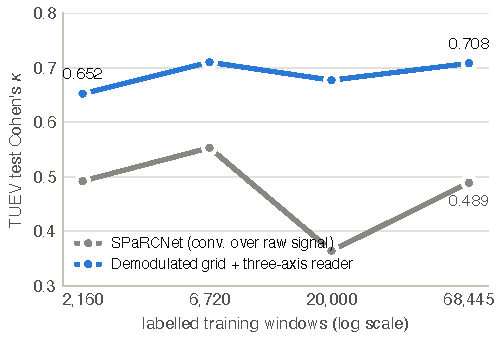
\includegraphics[width=\linewidth]{figures/fig2_label_curve.pdf}
\caption{TUEV test $\kappa$ against the number of labelled training windows (log axis, seed 0; full-data points are three-seed means). The demodulated grid keeps $\kappa$ 0.65 with 3\% of the labels, the sample-efficiency signature predicted in Section~\ref{sec:usable}; a convolutional model over the raw signal never reaches 0.56.}
\label{fig:curve}
\end{figure}

The real-data signature of T5 is already in the archive (Figure~\ref{fig:curve}): the envelope-token model trained on 2,160, 6,720, 20,000 and all 68,445 TUEV windows reaches $\kappa$ 0.652, 0.710, 0.677 and 0.708, while SPaRCNet reaches 0.492, 0.553, 0.364 and 0.489 (single seeds except the full-data cells). A 32-fold reduction of labels costs the demodulated model 0.056.

\subsection{Progressive attribution on clinical corpora}
\label{sec:attribution}

\subsubsection{Bands and factorization are the large effects (P1, P2)}
\label{sec:bands}
With raw band-limited waveform tokens and no transform, three seeds each (Table~\ref{tab:bands}), every paired difference is positive: one band to eight costs 0.42 AUC-PR on CHB-MIT and 0.11 on TUSZ, and a flat encoder costs 0.53 and 0.22. Independent ablations on an earlier frontend agree: removing the band attention axis cost 0.078 $\kappa$ on TUEV, 0.014 AUROC on TUAB and 0.010 AUC-PR on TUSZ; removing the physical electrode coordinates cost 0.080 on TUEV and 0.039 on TUSZ.

\begin{table}[t]
\centering
\TableStyle
\caption{Band decomposition and factorized attention with untransformed raw waveform tokens; three seeds, AUC-PR, per-seed paired differences in parentheses.}
\label{tab:bands}
\setlength{\tabcolsep}{3pt}
\begin{tabular}{@{}p{2.9cm}cc@{}}
\toprule
Contrast, all else equal & CHB-MIT & TUSZ \\
\midrule
1 band $\to$ 8 learned bands & 0.245 $\to$ 0.667 & 0.558 $\to$ 0.671 \\
 & (+0.39, +0.44, +0.43) & (+0.19, +0.12, +0.03) \\
flat (0.90M) $\to$ three-axis (1.62M) & 0.136 $\to$ 0.667 & 0.448 $\to$ 0.671 \\
 & (+0.59, +0.45, +0.56) & (+0.33, +0.18, +0.17) \\
\bottomrule
\end{tabular}
\end{table}

\subsubsection{Resolution must match the event (P6)}
On TUEV with envelope tokens and 8 bands, moving from 1\,s patches (5 per window) to 0.25\,s patches (20 per window) raises $\kappa$ from 0.627 to 0.708 over three seeds. The window over which the test direction $u$ of Section~\ref{sec:rotation} is measured is a separate parameter: with 0.25\,s tokens, lengthening it to 0.5 and 1\,s gives 0.649 and 0.611 at 8 bands, and at 16 bands under the stronger recipe it no longer matters (0.714, 0.739 and 0.737 for 0.25, 1 and 5\,s, seed 0). The resolution effect belongs to the token.

\subsubsection{Which view carries which label (P3, P4)}
\label{sec:views}
Figure~\ref{fig:content}a--b and Table~\ref{tab:views} hold the three-axis reader fixed and change what the token carries. On TUEV the envelope view is the whole story: it adds 0.17 to 0.20 over waveform tokens, and removing the waveform view from the full 16-band model costs 0.002. On CHB-MIT the waveform view is the whole story: envelope tokens alone fall 0.16 below waveform tokens, and removing the waveform view from the full model costs 0.167 (three-axis) and 0.062 (two-axis). The TUEV gain concentrates where Table~\ref{tab:labels} says it should. Per-class F1 over three seeds, waveform tokens to envelope-bearing tokens: GPED 0.55 $\to$ 0.82, PLED 0.52 $\to$ 0.61, ARTF 0.40 $\to$ 0.56, BCKG 0.88 $\to$ 0.92, while EYEM falls 0.57 $\to$ 0.31 and SPSW 0.16 $\to$ 0.00. Periodic discharges and artifact are envelope labels; eye movement and spike-and-wave are waveform labels, and envelope-only tokens lose them.

\begin{table}[t]
\centering
\TableStyle
\caption{Token content under the same three-axis reader. Three seeds unless a seed is given.}
\label{tab:views}
\setlength{\tabcolsep}{3pt}
\begin{tabular}{@{}lcc@{}}
\toprule
Token content & TUEV $\kappa$ & CHB-MIT AUC-PR \\
\midrule
waveform only (8 bands) & 0.536 & 0.667 \\
envelope only, rotated (8 bands) & 0.733 & 0.506 \\
both as separate rows (8 bands) & 0.690 & 0.699 \\
both in one token (16 bands), s0 / s2 & 0.714 / 0.716 & 0.697 / 0.710 \\
\quad envelope only, same model, s2 & 0.714 & 0.543 \\
\bottomrule
\end{tabular}
\end{table}

\begin{figure*}[t]
\centering
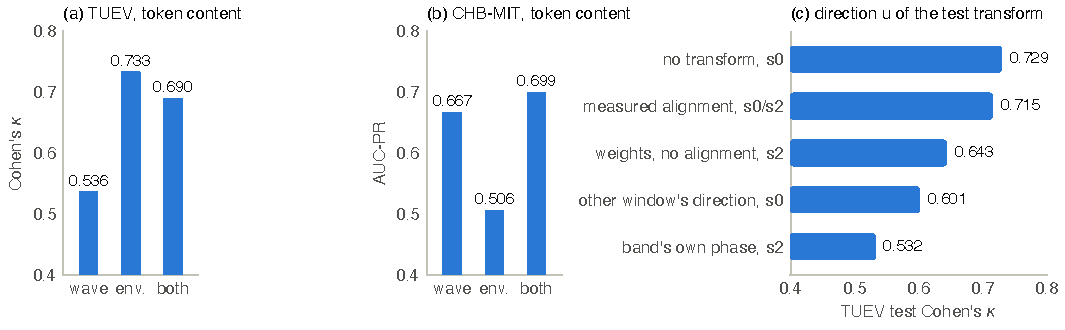
\includegraphics[width=\textwidth]{figures/fig3_content_and_rotation.pdf}
\caption{(a, b) Token content under the same three-axis reader, 8 learned bands, three seeds: TUEV needs the envelope view, CHB-MIT needs the waveform view. (c) The direction $u$ of the test transform on TUEV, 16-band three-axis model (seed in the label): the untransformed token and the measured content-independent direction sit together at the top; every direction that is uncorrelated with the content or carries the band's own phase costs 0.07 to 0.20, the ordering predicted in Section~\ref{sec:nuisance}.}
\label{fig:content}
\end{figure*}

\subsubsection{Physical bands versus learned rows (P5)}
\label{sec:rows}
A control that keeps the three-axis reader, the 16 rows, the recipe and the data but replaces the filterbank and demodulation with 16 learned linear views of each raw 0.25\,s patch completed on TUEV at seed 2 with test $\kappa$ 0.576 (balanced accuracy 0.552), against 0.711 for the unrotated band model and 0.716 for the rotated one at the same seed, a gap of 0.135. The learned-row model lands at the level of CBraMod trained from scratch (0.575) and below a one-row raw-patch control read by the two-axis encoder (0.638): a band axis over rows that are not physically distinct content is overhead, not structure. The CHB-MIT arm of this control is still training.

\subsubsection{Content-independent transforms (P7)}
\label{sec:rotation}
Pairing the token rotated by the measured direction against the untransformed token with the same data, recipe and initialisation (Supplementary Table~\ref{tab:rotation}) gives a mean difference of $-0.003$ over eight pairs (three-axis $-0.006$, two-axis $+0.001$). The entropy ladder of Figure~\ref{fig:content}c orders as predicted: the own-phase direction costs 0.03 to 0.24 relative to the measured one in 15 paired runs across four corpora (14 of 15 negative, mean $-0.076$), the weights-without-alignment variant 0.03 to 0.07 (three of three), another window's direction 0.11. The isometry-breaking variant, a bounded complex gain from a record-level statistic that makes the coupling linearly readable from the token ($R^2 = 0.98$ on synthetic signals), lowers TUEV from 0.693 to 0.660 at seed 0: readability of a quantity the labels are not a function of buys nothing. Inside a host that flattens the band axis into channels (BIOT's linear-attention transformer~\cite{yang2023biot} reading our frontend) the same rotation is not neutral: over three seeds, measured beats identity by 0.20 $\kappa$ on TUEV and by 0.12 on IIIC, and loses by 0.17 AUC-PR on CHB-MIT (Supplementary Table~\ref{tab:biot}). A transform the factorized reader undoes for free is, for a flattened reader, a feature with a task-dependent sign, which is what Section~\ref{sec:nuisance} predicts for a transform the reader cannot cheaply invert.

\subsubsection{The reader (Section~\ref{sec:factorized})}
\label{sec:reader}
Three-axis against two-axis at 16 bands under the same recipe, paired where seeds overlap: CHB-MIT $+0.089$ (two seeds), CAUEEG $+0.062$, IIIC $+0.057$, TUEP $+0.049$, TUEV $+0.016$ (two seeds), TUSZ $+0.016$, TUAR $+0.009$, ADFD $-0.017$; seven of eight positive, with 33\% more parameters, so the capacity confound remains open (Section~\ref{sec:limitations}). Two further results fix the reader's weight. A one-row raw-patch tokenizer read by the compact two-axis encoder reaches TUEV 0.638, above CBraMod's 12-layer encoder trained from scratch on the same arrays (0.575). CBraMod's own time-frequency stem read by the two-axis encoder reaches 0.738, the highest single-seed TUEV score in the archive, which is the first clause of P8.

\subsubsection{What did not matter}
Over the full ledger, other transforms from the same family (a non-isometric product form, an added coupling-strength feature, an own-band coupling term) differ from the untransformed token by at most 0.005 on average over 9 to 28 paired seeds; 8 versus 16 bands moves $+0.024$ with the sign changing by corpus; augmentation and weight decay move less than 0.01. Pretraining the model on amplitude reconstruction helped 3 of 12 corpora and hurt 9, consistent with the last clause of P8.

\subsection{Against baselines}
\label{sec:main}
The 1.6M model leads every reproduced baseline on the three event and seizure corpora whose protocols survive audit, TUEV, TUSZ and IIIC, and ties the strongest baseline on TUEP (Table~\ref{tab:main}). The first column is the main model of Section~\ref{sec:method}; where it has not been run, the same model with the rotated token stands in, and Supplementary Table~\ref{tab:rotation} shows the two differ by 0.003 on average. The TUEV from-scratch baselines were re-run in October 2026 with each author's native training code on the shared arrays, seed 0, validation-best checkpoints (CBraMod 0.575, EEG-Conformer 0.503, FFCL 0.459, BIOT 0.418, REVE 0.423); the pretrained rows use released weights with each repository's own preprocessing and were run under the earlier protocol. On TUEV the test set has 29,421 annotation rows over 3,243 distinct signals; weighting each distinct signal once gives 0.614 for our two-axis model, 0.576 for a raw-patch control and 0.547 for CBraMod, the same ordering with smaller margins. TUSZ is the cleanest win: the official evaluation split, three seeds on both sides, and a margin of 0.13 over FFCL obtained with raw band tokens alone.

\begin{table*}[t]
\centering
\TableStyle
\caption{Main comparison. Seed counts in parentheses; $\pm$ is the sample standard deviation over three seeds. From-scratch TUEV baselines: native training code, seed 0, validation-best checkpoint. Pretrained baselines: released weights, each repository's preprocessing. CHB-MIT is reported as open on the natural-grid protocol (Section~\ref{sec:protocols}).}
\label{tab:main}
\begin{tabular}{@{}>{\raggedright\arraybackslash}p{2.4cm}>{\raggedright\arraybackslash}p{3.0cm}>{\raggedright\arraybackslash}p{3.9cm}>{\raggedright\arraybackslash}p{3.2cm}>{\raggedright\arraybackslash}p{3.2cm}@{}}
\toprule
Corpus, metric & Main model & Same model, rotated token & Strongest from-scratch baseline & Strongest pretrained baseline \\
\midrule
TUEV, $\kappa$ & 0.729, 0.711 (2) & 0.693 $\pm$ 0.036 (3); 0.714, 0.716 (2) & CBraMod 0.575 (1) & REVE 0.685 $\pm$ 0.039 (3) \\
TUSZ, AUC-PR & 0.671 $\pm$ 0.032 (3, raw band tokens) & 0.680 $\pm$ 0.048 (3, two-axis); 0.674 (1) & FFCL 0.545 $\pm$ 0.030 (3) & EEGPT 0.545 $\pm$ 0.070 (3) \\
IIIC, $\kappa$ & not yet run & 0.524 (1); 0.497 $\pm$ 0.007 (3) & FFCL 0.423 $\pm$ 0.020 (3) & REVE 0.436 $\pm$ 0.003 (3) \\
TUEP, AUROC & not yet run & 0.811 (1); 0.810 $\pm$ 0.004 (3, 8 bands) & EEGPT 0.786 $\pm$ 0.021 (3) & LaBraM 0.778 $\pm$ 0.019 (3) \\
CHB-MIT, AUC-PR & open (natural grid) & open (natural grid) & CBraMod 0.570 (1, natural grid) & EEGPT 0.379 (1, natural grid) \\
Sleep-EDF, $\kappa$ & not yet run & 0.700 (1) & ContraWR 0.692 $\pm$ 0.015 (3) & CBraMod 0.672 $\pm$ 0.005 (3) \\
TUAR, $\kappa$ & not yet run & 0.724 (1) & CNN-Transformer 0.712 (1) & CBraMod 0.715 (1) \\
CAUEEG, bal.\ acc. & not yet run & 0.543 (1) & BIOT 0.561 $\pm$ 0.012 (3) & EEGPT 0.547 $\pm$ 0.021 (3) \\
ADFD, bal.\ acc. & not yet run & 0.460 (1) & BIOT 0.525 $\pm$ 0.021 (3) & REVE 0.501 $\pm$ 0.049 (3) \\
\bottomrule
\end{tabular}
\end{table*}

\paragraph{CHB-MIT.}
The evaluation set used throughout our archive added 162 seizure-centred positive windows to the natural 10\,s grid (276 positives against 114); TFM-Tokenizer's released CHB-MIT script likewise adds seizure-centred positives in every split. The same saved predictions score 0.697 on the enriched set and 0.486 on the natural grid; the strongest baseline reproduced on the natural grid with native code is CBraMod at 0.570. Our model has not completed a run on the natural-grid split (the first attempt stopped at validation AUC-PR 0.416 against 0.564 on the enriched split), so CHB-MIT is open and will be reported on the natural grid for every model or not at all; the published TFM-Tokenizer figure of 0.627 is not comparable to either set.
